% =====================================================================
%  StockIT — Detailed presentation report (English version)
%  Compile with : pdflatex rapport_presentation_en.tex  (twice for ToC)
%  Tested on Overleaf (pdfLaTeX) and TeX Live.
% =====================================================================
\documentclass[11pt,a4paper]{article}

% ---- Encoding & language -------------------------------------------
\usepackage[utf8]{inputenc}
\usepackage[T1]{fontenc}
\usepackage[english]{babel}
\usepackage{lmodern}
\usepackage{microtype}

% ---- Page layout ---------------------------------------------------
\usepackage[a4paper,margin=2.2cm,top=2cm,bottom=2cm]{geometry}
\usepackage{parskip}
\setlength{\parskip}{4pt}
\setlength{\parindent}{0pt}

% ---- Extensions ----------------------------------------------------
\usepackage{xcolor}
\definecolor{primary}{HTML}{1F4E79}
\definecolor{accent}{HTML}{C0504D}
\definecolor{soft}{HTML}{E8EEF7}
\definecolor{softgrey}{HTML}{F5F5F5}
\definecolor{green1}{HTML}{2E7D32}
\definecolor{orange1}{HTML}{E65100}

\usepackage{enumitem}
\setlist[itemize]{leftmargin=1.3em,itemsep=2pt,topsep=3pt}
\setlist[enumerate]{leftmargin=1.5em,itemsep=2pt,topsep=3pt}

\usepackage{tcolorbox}
\tcbuselibrary{skins,breakable}

\usepackage{tikz}
\usetikzlibrary{arrows.meta,positioning,shapes.geometric,shadows,fit,backgrounds}

\usepackage{booktabs}
\usepackage{array}
\usepackage{tabularx}
\newcolumntype{L}[1]{>{\raggedright\arraybackslash}p{#1}}

\usepackage{titlesec}
\titleformat{\section}
  {\normalfont\Large\bfseries\color{primary}}
  {\thesection.}{0.6em}{}
\titleformat{\subsection}
  {\normalfont\large\bfseries\color{primary!85!black}}
  {\thesubsection}{0.6em}{}
\titleformat{\subsubsection}
  {\normalfont\normalsize\bfseries\color{accent}}
  {}{0em}{}
\titlespacing*{\section}{0pt}{14pt}{6pt}
\titlespacing*{\subsection}{0pt}{10pt}{4pt}
\titlespacing*{\subsubsection}{0pt}{6pt}{2pt}

\usepackage{fancyhdr}
\pagestyle{fancy}
\fancyhf{}
\renewcommand{\headrulewidth}{0.3pt}
\renewcommand{\footrulewidth}{0pt}
\fancyhead[L]{\small\color{primary!80!black}\textbf{StockIT} — Presentation report}
\fancyhead[R]{\small\color{black!60}\thepage}

\usepackage[hidelinks,colorlinks=true,linkcolor=primary,urlcolor=primary]{hyperref}

% ---- TikZ styles ---------------------------------------------------
\tikzset{
  box/.style   = {rectangle, rounded corners=4pt, draw=primary,
                  fill=soft, minimum height=11mm, minimum width=26mm,
                  align=center, font=\small},
  cbox/.style  = {rectangle, rounded corners=4pt, draw=orange1,
                  fill=orange!10, minimum height=11mm, minimum width=30mm,
                  align=center, font=\small},
  aibox/.style = {rectangle, rounded corners=4pt, draw=accent,
                  fill=red!5, minimum height=11mm, minimum width=30mm,
                  align=center, font=\small},
  layer/.style = {rectangle, rounded corners=3pt, draw=primary!70,
                  fill=soft, minimum height=8mm, minimum width=42mm,
                  align=center, font=\small},
  arr/.style   = {-{Latex[length=2.5mm]}, thick, draw=black!55}
}

% ---- Reusable boxes ------------------------------------------------
\newtcolorbox{infobox}[1][]{
  enhanced, colback=soft, colframe=primary,
  boxrule=0.4pt, arc=3pt, left=8pt, right=8pt, top=5pt, bottom=5pt,
  fonttitle=\bfseries\color{white},
  coltitle=white, colbacktitle=primary,
  title=#1, breakable}

\newtcolorbox{warnbox}[1][]{
  enhanced, colback=orange!5, colframe=orange1,
  boxrule=0.4pt, arc=3pt, left=8pt, right=8pt, top=5pt, bottom=5pt,
  fonttitle=\bfseries, coltitle=white, colbacktitle=orange1,
  title=#1, breakable}

\newtcolorbox{ideabox}[1][]{
  enhanced, colback=green!4, colframe=green1,
  boxrule=0.4pt, arc=3pt, left=8pt, right=8pt, top=5pt, bottom=5pt,
  fonttitle=\bfseries, coltitle=white, colbacktitle=green1,
  title=#1, breakable}

% =====================================================================
\begin{document}

% ---------- Cover page ----------------------------------------------
\thispagestyle{empty}
\begin{center}
\vspace*{1.5cm}
{\color{primary}\rule{\linewidth}{1.2pt}}\\[6pt]
{\Huge\bfseries\color{primary} StockIT}\\[6pt]
{\Large\itshape An intelligent mobile app for\\
IT stock management, powered by AI}\\[4pt]
{\color{primary}\rule{\linewidth}{1.2pt}}

\vspace{2.5cm}

\begin{tcolorbox}[colback=soft, colframe=primary,
  boxrule=0.5pt, arc=5pt, width=0.85\linewidth, halign=center]
\Large\bfseries Detailed presentation report\\[4pt]
\normalsize\normalfont
Architecture, features, workflows,\\
automation and integrations
\end{tcolorbox}

\vspace{3cm}

\begin{tabular}{rl}
\textbf{Platform}       & Android (Java, min SDK~26 — Android~8)\\[3pt]
\textbf{Domain}         & IT Logistics / Supply Chain\\[3pt]
\textbf{Intelligence}   & Vision + OCR + LLM (multi-level cascade)\\[3pt]
\textbf{Integrations}   & Jira Cloud, Slack, Firebase, SendGrid\\[3pt]
\textbf{Date}           & \today
\end{tabular}

\vfill
{\color{primary!70}\small Document prepared for mentor presentation / thesis defense}
\end{center}

\newpage

% ---------- Table of contents ---------------------------------------
\tableofcontents
\newpage

% =====================================================================
\section{Introduction \& context}

\textbf{StockIT} is an Android application designed to digitize and
automate the management of an IT hardware inventory for a logistics
team. It replaces manual processes (Excel sheets, repetitive typing,
paper labels) with a \emph{scan + AI} flow that drastically reduces
the time needed to receive or hand out equipment.

\begin{infobox}[Problem addressed]
The logistics department receives boxes of IT equipment every week
(monitors, keyboards, mice, laptops\dots). Each item must be~:
\begin{itemize}
  \item linked to a purchase order (PO) and to an invoice;
  \item recorded in stock with all its attributes;
  \item then assigned to a support ticket opened by a colleague.
\end{itemize}
Done manually, these steps are \textbf{slow, error-prone and hard
to trace}. StockIT automates the entire chain.
\end{infobox}

\subsection{Goals}
\begin{itemize}
  \item \textbf{Zero double entry} thanks to OCR and computer vision.
  \item \textbf{Full traceability}: every movement is logged and
        notified in real time.
  \item \textbf{AI assistance} to identify products, read invoices,
        pick the right ticket, and answer questions.
  \item \textbf{Offline resilience}: critical features keep working
        with no network.
\end{itemize}

% =====================================================================
\section{Overall architecture}

\subsection{Layered view}

\begin{center}
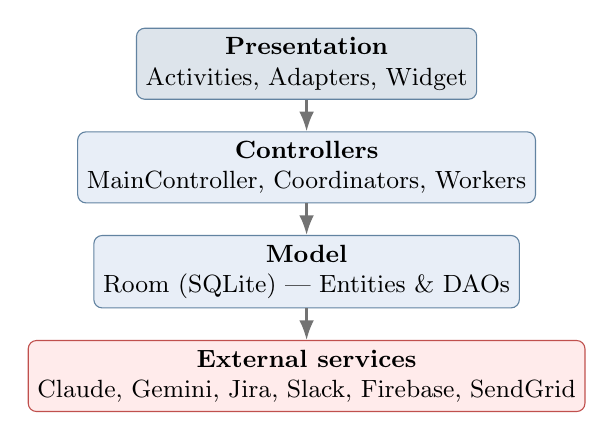
\begin{tikzpicture}[node distance=4mm]
  \node[layer, fill=primary!15] (ui) {\textbf{Presentation}\\Activities, Adapters, Widget};
  \node[layer, below=of ui]      (ctl){\textbf{Controllers}\\MainController, Coordinators, Workers};
  \node[layer, below=of ctl]     (mdl){\textbf{Model}\\Room (SQLite) — Entities \& DAOs};
  \node[layer, below=of mdl, fill=red!8, draw=accent] (svc){\textbf{External services}\\Claude, Gemini, Jira, Slack, Firebase, SendGrid};
  \foreach \a/\b in {ui/ctl,ctl/mdl,mdl/svc}
    \draw[arr] (\a) -- (\b);
\end{tikzpicture}
\end{center}

\subsection{Project key figures}

\begin{center}
\begin{tabular}{lr}
\toprule
\textbf{Item} & \textbf{Volume} \\
\midrule
Screens (Android Activities)             & \textbf{15} \\
Adapters \& UI controllers               & \textbf{18} \\
Persisted entities (Room)                & \textbf{13} \\
Integrated external services             & \textbf{9}  \\
Fallback levels in the AI cascade        & \textbf{5}  \\
Database schema version                  & \textbf{22} \\
\bottomrule
\end{tabular}
\end{center}

% =====================================================================
\section{Feature overview}

\subsection{Main screens}

\begin{tabularx}{\linewidth}{@{}lX@{}}
\toprule
\textbf{Screen} & \textbf{Role}\\
\midrule
\textit{Login}                & Password or biometric sign-in, with 3 roles (Admin, Manager, Viewer). \\
\textit{Dashboard}            & Central control panel: stock, purchases, reports, audit, users, AI, leaderboard. \\
\textit{Scan asset}           & Photo capture + automatic equipment type recognition. \\
\textit{Batch scan}           & Continuous multi-barcode detection through the camera. \\
\textit{Receive package}      & Photo of the delivery note / invoice with structured extraction. \\
\textit{PO selection}         & Pick the right purchase order among those detected on the invoice. \\
\textit{Package label}        & Automatic reading of reference, quantity, brand, printed PO. \\
\textit{Scan out}             & Hand out equipment with a choice of ticket-assignment mode. \\
\textit{Ticket list}          & Search and pick an open Jira ticket. \\
\textit{AI assistant}         & Natural-language chat about the state of the stock. \\
\textit{Claims}               & Internal complaint follow-up (open / in progress / resolved). \\
\textit{Profile}              & Profile editing, points, badges and history. \\
\textit{Home widget}          & Android home-screen tile showing the current item count, refreshed automatically. \\
\bottomrule
\end{tabularx}

\subsection{Features grouped by theme}

\begin{center}
\begin{tabularx}{\linewidth}{@{}lX@{}}
\toprule
\textbf{Theme} & \textbf{Features}\\
\midrule
\textbf{Intake}          & Invoice scan, PO/supplier extraction, label cross-check, automatic stock entry.\\
\textbf{Handout}         & Product scan, quantity input, 3 ticket-assignment modes, stock decrement.\\
\textbf{Jira tickets}    & Read, filter, select, auto-create on anomalies.\\
\textbf{AI assistant}    & Q\&A in natural language about the stock, inventory context injected.\\
\textbf{Claims}          & Prioritized form (Low / Medium / High) + status tracking.\\
\textbf{Users}           & Roles, biometric auth, gamification (points, badges, quests).\\
\textbf{Dashboard}       & KPIs, trend charts, items below threshold, history.\\
\textbf{Widget}          & Real-time tile on the Android home screen.\\
\textbf{Notifications}   & FCM push + Slack alerts on every critical movement.\\
\textbf{Reports}         & Monthly PDF automatically generated and emailed.\\
\textbf{Batch scan}      & Continuous multi-barcode detection through the camera.\\
\textbf{Audit \& logs}   & Every action logged with user, timestamp, device.\\
\textbf{Gamification}    & Quests, points, badges, user leaderboard.\\
\bottomrule
\end{tabularx}
\end{center}

% =====================================================================
\section{\textsc{Intake} workflow — receiving an item}

\begin{infobox}[Goal]
Identify the received equipment, link it to its purchase order and
invoice, then register it in stock — all in a few photos.
\end{infobox}

\begin{enumerate}
  \item \textbf{Scan the product.} The technician takes a photo of
        the item. The AI automatically recognizes the equipment type
        (monitor, keyboard, mouse\dots).
  \item \textbf{Scan the invoice / delivery note.} A second photo is
        used to extract, by text recognition, the supplier and the
        list of purchase orders that appear on the document.
  \item \textbf{Pick the purchase order.} The app displays the
        detected POs and highlights the one that matches the scanned
        product (\emph{Already in DB}, \emph{Matches the scan}).
  \item \textbf{Scan the box label.} Quantity, article number and
        brand are read automatically, then compared to the selected PO.
  \item \textbf{Register in stock.} The intake is confirmed: stock is
        updated, a trace is kept in the history, and a notification
        is sent to the team.
\end{enumerate}

\begin{center}
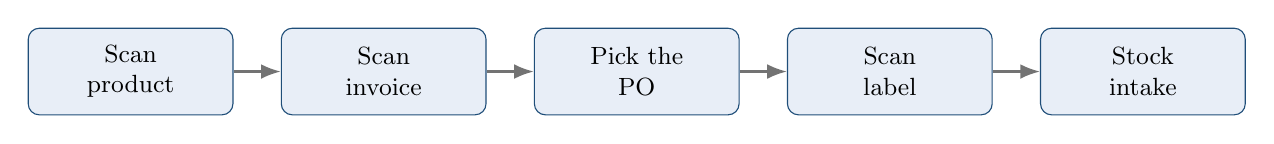
\begin{tikzpicture}[node distance=5mm and 6mm]
  \node[box] (n1) {Scan\\product};
  \node[box, right=of n1] (n2) {Scan\\invoice};
  \node[box, right=of n2] (n3) {Pick the\\PO};
  \node[box, right=of n3] (n4) {Scan\\label};
  \node[box, right=of n4] (n5) {Stock\\intake};
  \foreach \a/\b in {n1/n2,n2/n3,n3/n4,n4/n5}
    \draw[arr] (\a) -- (\b);
\end{tikzpicture}
\end{center}

% =====================================================================
\section{\textsc{Handout} workflow — ticket assignment}

\begin{infobox}[Goal]
Take one or more items out of stock and trace each unit to its
recipient through one of the \textbf{three assignment modes}.
\end{infobox}

\begin{enumerate}
  \item \textbf{Scan the product to hand out}: the AI identifies the
        equipment.
  \item \textbf{Enter the quantity}: checked against available stock.
  \item \textbf{Pick the assignment mode}: for each unit, the user
        chooses one of the three modes below.
\end{enumerate}

\vspace{4pt}
\begin{center}
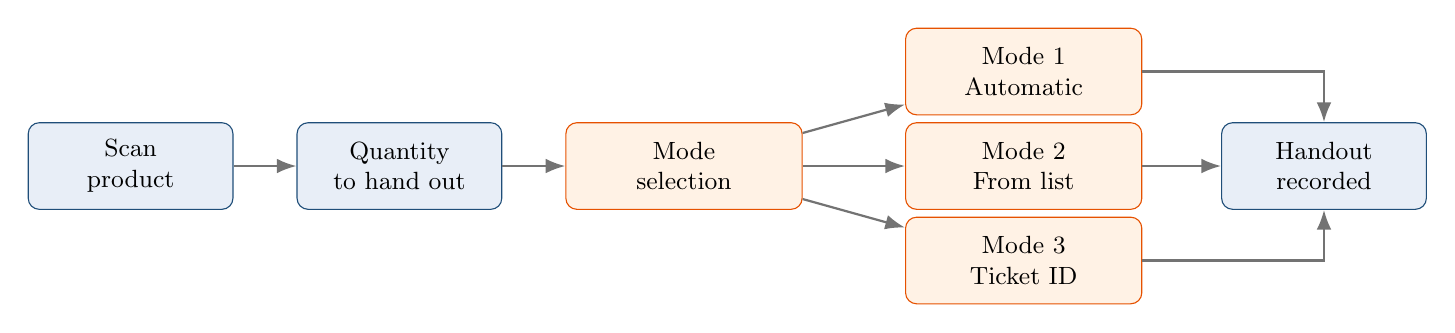
\begin{tikzpicture}[node distance=5mm and 8mm]
  \node[box] (s1) {Scan\\product};
  \node[box, right=of s1] (s2) {Quantity\\to hand out};
  \node[cbox, right=of s2] (s3) {Mode\\selection};
  \node[cbox, right=13mm of s3, yshift=12mm] (m1) {Mode 1\\Automatic};
  \node[cbox, right=13mm of s3]              (m2) {Mode 2\\From list};
  \node[cbox, right=13mm of s3, yshift=-12mm] (m3) {Mode 3\\Ticket ID};
  \node[box,  right=10mm of m2]              (out) {Handout\\recorded};
  \draw[arr] (s1) -- (s2);
  \draw[arr] (s2) -- (s3);
  \draw[arr] (s3) -- (m1);
  \draw[arr] (s3) -- (m2);
  \draw[arr] (s3) -- (m3);
  \draw[arr] (m1.east) -| (out.north);
  \draw[arr] (m2)      -- (out);
  \draw[arr] (m3.east) -| (out.south);
\end{tikzpicture}
\end{center}

\subsection{The 3 assignment modes}

\begin{center}
\begin{tabularx}{\linewidth}{@{}lX@{}}
\toprule
\textbf{Mode}            & \textbf{Description}\\
\midrule
\textbf{1. Automatic (AI)} & The app suggests the most relevant ticket
    itself by analyzing open requests (summary, priority, due date)
    and matching them against the scanned product.\\
\addlinespace
\textbf{2. From list}     & The technician browses the open tickets,
    filters by keyword or priority, and manually selects the right
    one.\\
\addlinespace
\textbf{3. Ticket ID}     & The technician types a known ticket ID
    directly; the app verifies that it exists before confirming.\\
\bottomrule
\end{tabularx}
\end{center}

\begin{enumerate}\setcounter{enumi}{3}
  \item \textbf{Confirmation}: the handout is recorded with the link
        to the chosen ticket and the loop continues until every unit
        has been assigned.
  \item \textbf{Closing}: on-screen summary + automatic team
        notification.
\end{enumerate}

% =====================================================================
\section{The AI cascade — never blocking}

Every recognition call goes through 5 successive levels. As soon as
one level answers, the following ones are not queried. The last
level runs \textbf{100\,\% locally}, guaranteeing that the app keeps
working with no network.

\begin{center}
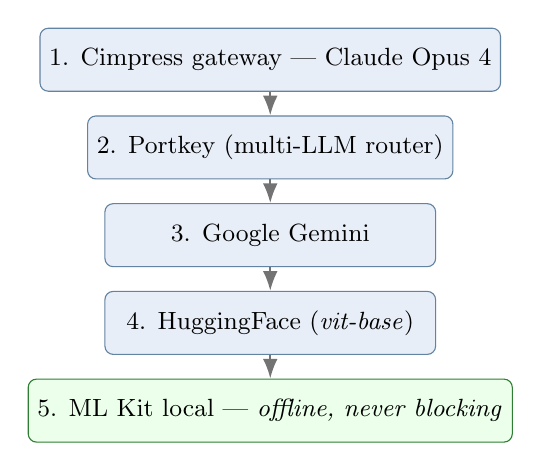
\begin{tikzpicture}[node distance=3mm]
  \node[layer] (l1) {1. Cimpress gateway — Claude Opus~4};
  \node[layer, below=of l1] (l2) {2. Portkey (multi-LLM router)};
  \node[layer, below=of l2] (l3) {3. Google Gemini};
  \node[layer, below=of l3] (l4) {4. HuggingFace (\emph{vit-base})};
  \node[layer, below=of l4, fill=green!8, draw=green1]
       (l5) {5. ML~Kit local — \emph{offline, never blocking}};
  \foreach \a/\b in {l1/l2,l2/l3,l3/l4,l4/l5}
    \draw[arr] (\a) -- (\b);
\end{tikzpicture}
\end{center}

\begin{ideabox}[Why this cascade?]
\begin{itemize}
  \item \textbf{Quality} peaks at the top of the chain (state-of-the-art
        vision LLM).
  \item \textbf{Resilience}: network outage, quota exceeded, API error —
        a lower level always takes over.
  \item \textbf{Controlled cost}: the free levels (ML~Kit) act as a
        safety net, not as the main option.
\end{itemize}
\end{ideabox}

% =====================================================================
\section{Automation \& smart scenarios}

\subsection{Anti-forgetting kit check}
When a \textbf{monitor} is received, a dialog forces the technician
to check the mandatory accessories: \emph{power cable} and
\emph{HDMI cable}. If any is missing, a Slack alert is sent and a
Jira anomaly ticket is created automatically — without blocking the
stock entry.

\subsection{Auto-matching ticket $\leftrightarrow$ product}
In the automatic handout mode, the AI receives the list of open
tickets (summary, priority, due date) and the scanned equipment,
then returns a unit split that respects priority and deadlines.

\subsection{Automatic Jira ticket creation}
Three triggers:
\begin{itemize}
  \item Incomplete accessory kit (monitor without its cables).
  \item An item's stock below its critical threshold.
  \item A purchase order not received after a given delay.
\end{itemize}

\subsection{Context-aware Slack notifications}
Every action produces a targeted message:
\begin{itemize}
  \item Success: \emph{``[OK] Handout recorded — 3 keyboards to TICKET-42''}
  \item Anomaly: \emph{``[WARN] Incomplete kit — monitor without HDMI cable''}
  \item Report: \emph{``[INFO] Monthly report ready, 145 items''}
\end{itemize}

\subsection{Scheduled PDF reports}
A background task (WorkManager) runs on a configurable schedule: it
collects the current stock state, generates a summary PDF (with an
AI-written recap) and emails it through SendGrid — even when the app
is closed.

\subsection{Image optimization before AI}
Photos are compressed to 1024\,px at 85\,\% quality before being
sent to the vision models — lower latency and controlled bandwidth
usage.

\subsection{Consistency check: invoice PO $\leftrightarrow$ label PO}
The PO printed on the box label is compared with the PO selected on
the invoice. A non-blocking warning is displayed if they disagree.

\subsection{Real-time widget refresh}
Every stock movement triggers a refresh of the home-screen widget:
the tile always shows the exact counter.

\subsection{Gamification}
Every scan and every user action awards points and badges, and feeds
a quest system with a leaderboard.

% =====================================================================
\section{Data model}

\begin{center}
\begin{tabularx}{\linewidth}{@{}lX@{}}
\toprule
\textbf{Entity} & \textbf{Role}\\
\midrule
\textit{Product}          & Item in stock (name, category, quantity, threshold, brand\dots)\\
\textit{PurchaseOrder}    & Purchase order (supplier, quantity, status)\\
\textit{ShippingOrder}    & Outbound shipment \\
\textit{StockMovement}    & Intake / handout (product, quantity, linked ticket, reason)\\
\textit{Category}         & Product category \\
\textit{Supplier}         & Supplier \\
\textit{User}             & User (role, points, badges, level)\\
\textit{AuditLog}         & Audit trail of every action \\
\textit{Claim}            & Complaint (subject, priority, status)\\
\textit{Quest}            & Gamification quest (goal, progress, reward)\\
\textit{AnalyzedTicket}   & Local cache of an analyzed Jira ticket \\
\textit{ChatMessage}      & AI assistant message \\
\textit{AIInsight}        & Recommendation or anomaly detected by the AI \\
\bottomrule
\end{tabularx}
\end{center}

% =====================================================================
\section{Integrations \& external services}

\begin{center}
\begin{tabularx}{\linewidth}{@{}lXl@{}}
\toprule
\textbf{Service} & \textbf{Usage} & \textbf{Auth}\\
\midrule
Cimpress gateway (Claude Opus~4)  & Product vision, invoice extraction, ticket matching & Bearer token \\
Portkey                           & Secondary LLM router (chat, fallback) & API key \\
Google Gemini                     & Vision fallback & API key \\
HuggingFace (\emph{vit-base})     & Image classification fallback & Bearer token \\
ML~Kit (Google, local)            & OCR, barcodes, offline image labeling & --- \\
Jira Cloud REST v3                & Read and create tickets & Basic (email + token) \\
Firebase Cloud Messaging          & Real-time push notifications & Service account \\
Slack \emph{Incoming Webhooks}    & Automatic team alerts & Webhook URL \\
SendGrid                          & PDF report delivery by email & API key \\
\bottomrule
\end{tabularx}
\end{center}

% =====================================================================
\section{Tools \& libraries used}

\begin{tabularx}{\linewidth}{@{}lX@{}}
\toprule
\textbf{Category} & \textbf{Technologies}\\
\midrule
\textbf{Language \& build}      & Java 11, Gradle Kotlin DSL, Android Gradle Plugin, min~SDK~26, target~SDK~35 \\
\textbf{UI}                     & Material Design, AppCompat, RecyclerView, ConstraintLayout, CardView, DrawerLayout, MPAndroidChart (charts)\\
\textbf{Camera \& vision}       & CameraX (core, camera2, lifecycle, view), ML~Kit (Text Recognition, Barcode Scanning, Image Labeling, Object Detection)\\
\textbf{AI / LLM}               & OkHttp calls to Claude, Gemini, Portkey, HuggingFace; Google Generative AI SDK\\
\textbf{Database}               & Room (SQLite), schema version 22 \\
\textbf{Networking}             & OkHttp, Retrofit, Gson\\
\textbf{Cloud backend}          & Firebase BoM (Messaging, optional Firestore)\\
\textbf{PDF \& reports}         & iText 7 (\emph{itext7-core}) \\
\textbf{Email}                  & SendGrid Java SDK \\
\textbf{Background jobs}        & WorkManager (PeriodicWorkRequest) \\
\textbf{Widget}                 & AppWidgetProvider (Android framework) \\
\textbf{Authentication}         & AndroidX Biometric (fingerprint / face) \\
\textbf{Testing}                & JUnit 4, AndroidX Test, Espresso \\
\bottomrule
\end{tabularx}

% =====================================================================
\section{Security \& best practices}

\subsection{Secret management}
API keys are injected into \emph{BuildConfig} at compile time, sourced
from environment variables (\emph{set\_env.ps1} / \emph{.env.sh} files
that are not versioned). No secret is stored in clear text in the Git
repository.

\subsection{Authentication}
Two modes: password and biometric (via the AndroidX Biometric API).
Three application-level roles: \emph{Admin}, \emph{Manager},
\emph{Viewer}.

\subsection{Traceability}
Every user action is written to an audit table (user, action,
timestamp, device) — read-only from the UI. That table also feeds
the \emph{Audit} tab of the dashboard.

\subsection{Android permissions}
Camera, Internet, Network state, Notifications, Biometric — all
requested at runtime and strictly limited to their required use.

\subsection{Networking}
Explicit timeouts (connect 10\,s, read 30\,s+), HTTPS everywhere,
defensive error handling (no crash on AI failure — the cascade takes
over).

% =====================================================================
\section{Added value \& innovations}

\begin{ideabox}[Differentiators]
\begin{enumerate}
  \item \textbf{5-level AI cascade, never blocking} — the app keeps
        running even offline.
  \item \textbf{Zero double entry} — vision + OCR everywhere:
        invoices, labels, products.
  \item \textbf{Smart ticket $\leftrightarrow$ item assignment} —
        automatic prioritization by urgency and deadline.
  \item \textbf{Full traceability} — audit + Slack + Jira in sync on
        every action.
  \item \textbf{Embedded AI assistant} — natural-language questions
        on stock state.
  \item \textbf{Anti-forgetting kit check} — mandatory accessory
        verification (cables) on monitors.
  \item \textbf{Scheduled PDF reports} automatically emailed
        (WorkManager + SendGrid).
  \item \textbf{Home widget} refreshed after every stock movement.
  \item \textbf{Gamification} — quests, points and badges to keep
        logistics users engaged.
\end{enumerate}
\end{ideabox}

% =====================================================================
\section{Conclusion}

StockIT proves that a well-designed mobile application can replace,
on its own, a whole set of manual processes involved in managing an
IT hardware inventory. By combining \textbf{computer vision},
\textbf{local OCR}, \textbf{business integrations} (Jira, Slack) and
\textbf{background automation}, it saves the logistics team a lot of
time while providing complete traceability.

The modular architecture (swappable AI cascade, extensible Room
entities, decoupled external services) makes it easy to add new
features later: Zycus purchase-request ingestion, consumption
forecasting, or ERP integration.

\vspace{6pt}
\begin{center}
\color{primary!70}\itshape\small
End of report — thank you for your attention.
\end{center}

\end{document}
